\documentclass{article}
\usepackage{ctex}
\usepackage{graphicx}

\title{ResNet-18与CIFAR-100}
\author{王逸群 19307110397}
\date{2022.4.17}

\begin{document}

\maketitle

GitHub repo 链接:https://github.com/quniLcs/cv-mid

网盘链接:

\section{实验设置}

\subsection{数据集}

本项目使用CIFAR-100数据集,
其中包含60000张$32\times32$的彩色图片,
其中训练集50000张,测试集10000张,
被平均分为100类。

\subsection{网络结构}

本项目使用ResNet-18网络结构,
其中激活函数为ReLU,
最大的特征为残差连接。
后者包括两种单元结构如图\ref{fig:GraphI}和图\ref{fig:GraphII}所示。

\begin{figure}[p]
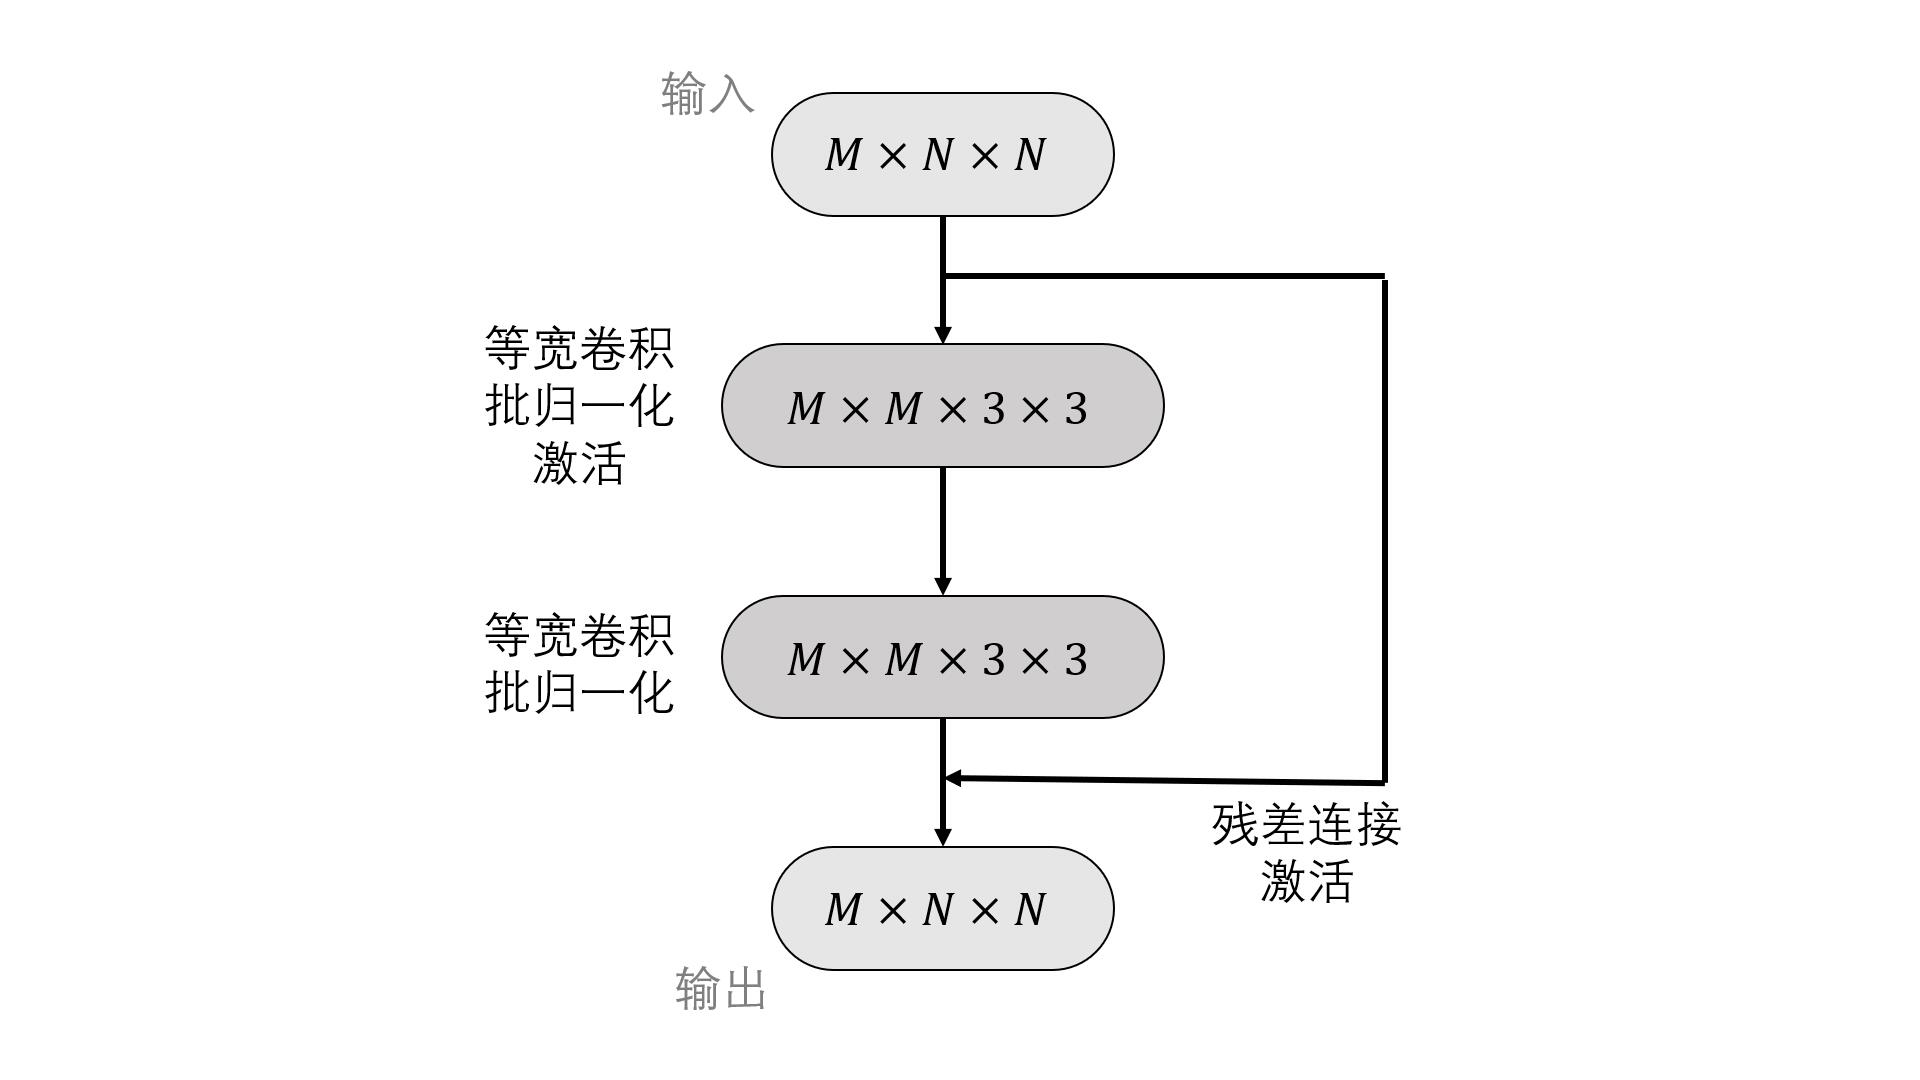
\includegraphics[width=\linewidth]{graph/I.jpg}
\caption{残差连接第一种单元结构}
\label{fig:GraphI}
\end{figure}

\begin{figure}[p]
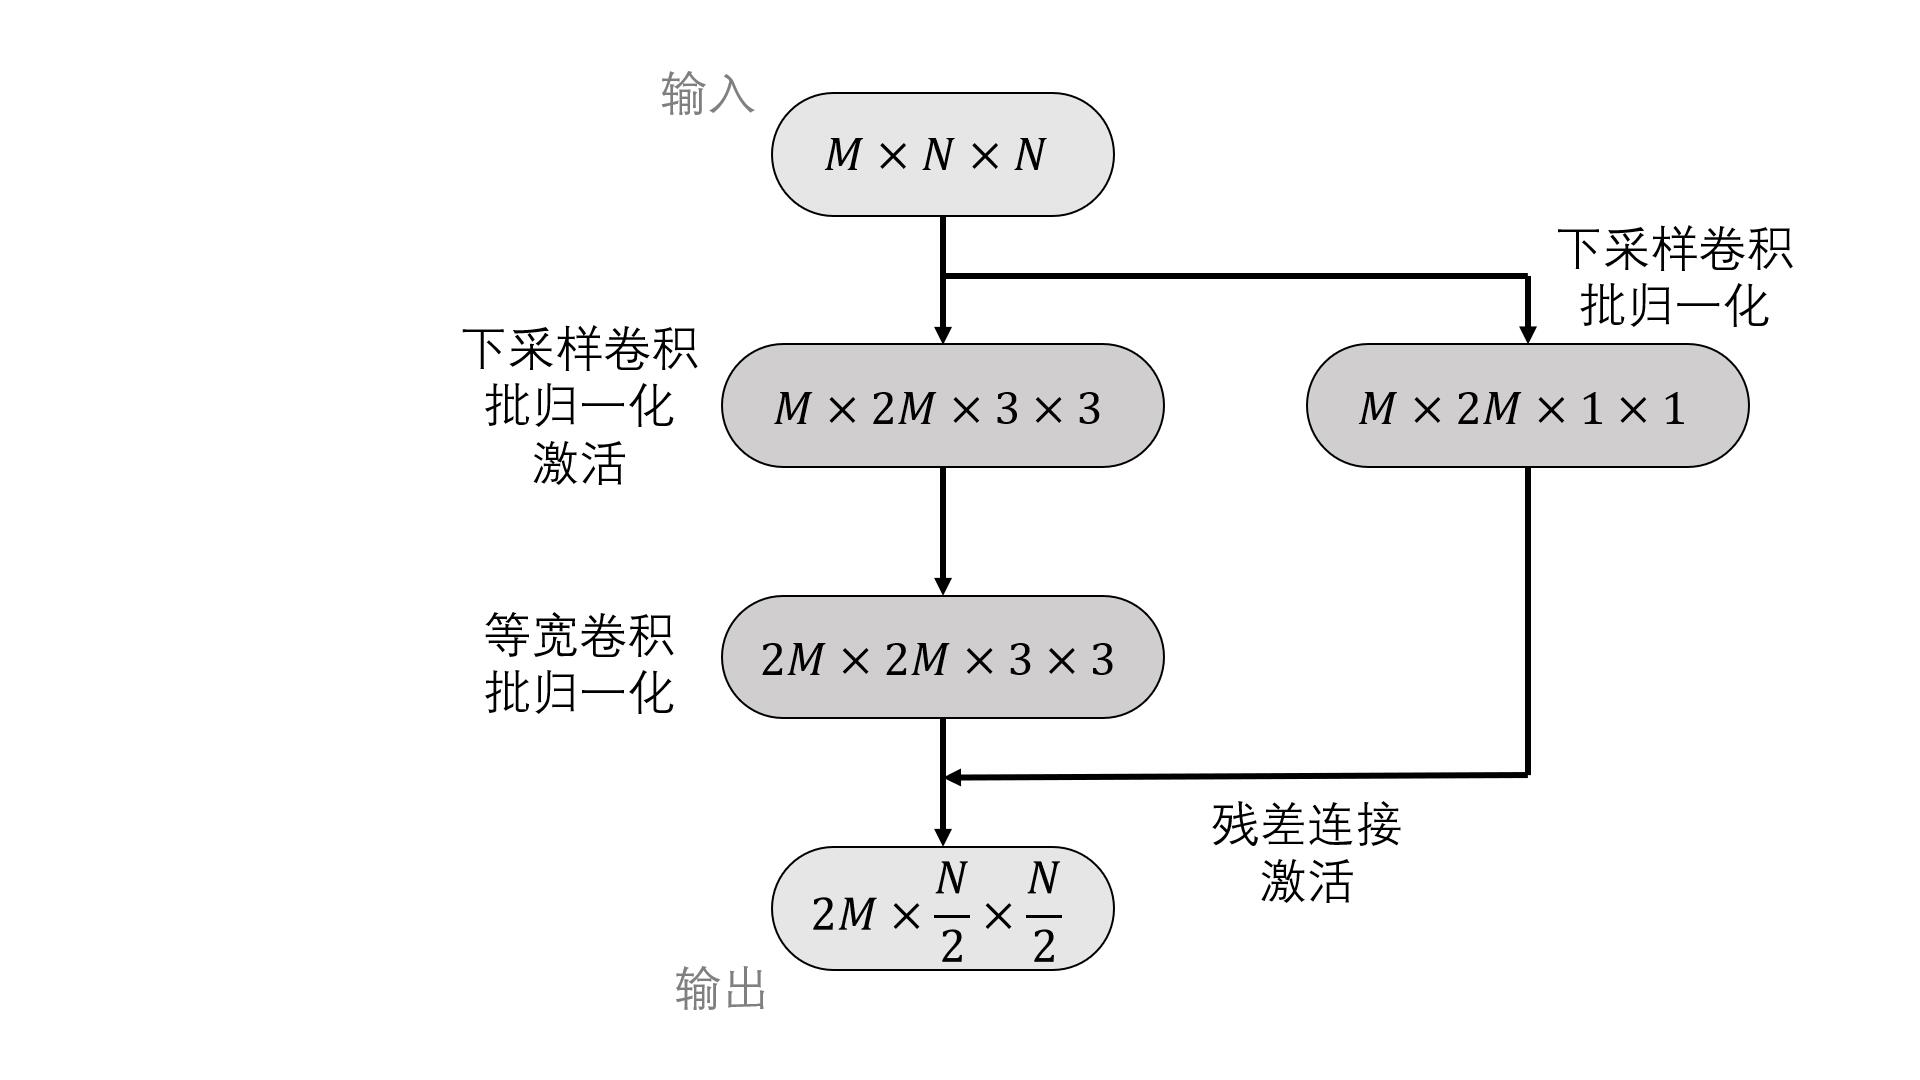
\includegraphics[width=\linewidth]{graph/II.jpg}
\caption{残差连接第二种单元结构}
\label{fig:GraphII}
\end{figure}

对于输入的图像,
先进行步长为2的$3\times64\times7\times7$卷积操作,
并进行批归一化和激活,
维度变为$64\times16\times16$;
再进行步长为2的$3\times3$池化操作,
维度变为$64\times8\times8$;
接着通过两次第一种单元结构,维度不变;
再通过第二种单元结构,维度变为$128\times4\times4$;
再通过第一种单元结构,维度不变;
再通过第二种单元结构,维度变为$256\times2\times2$;
再通过第一种单元结构,维度不变;
再通过第二种单元结构,维度变为$512\times1\times1$;
再通过第一种单元结构,维度不变;
最后通过全连接得到输出。

\subsection{超参数设置}

参数初始化:MSRA;

学习率:由0.1阶梯下降至0.001;

优化器:Adam;

回合数:30;

批量大小:128;

每回合循环数:391;

总循环数:$ 30 \times 391 = 11730 $;

损失函数:交叉熵损失函数;

评价指标:精确度。

\section{Baseline}

\section{Cutmix}

\section{Cutout}

\section{Mixup}

\end{document}